\chapter{Pose estimation III: Relative pose from real data}

Now knowing that a neural network given known 2D coordinates of features can
find the 3D relative pose, experiments were done using RGB images and ground
truth labels collected on a real robotic system.

\section{Method}

RGB images were collected while executing the pushing policy on one of the
robots. The images were labeled with relative poses to the end-effector using
the position estimates of the cube using the LiDAR, and the arm using the
forward kinematics on the servo angles. The camera was placed at random
positions around the workspace, always capturing at least the portion of the
arm as shown in figure \ref{fig:end-effector-frame}, and capturing at least the
top surface of the cube. Distracting objects were put into the scene such as
different kinds of rubble in the background, changing the appearance of the
table surface, changing light conditions, and playing up videos in the
background. Some of the training images are shown in figure
\ref{fig:relpose-training-data}. Images were augmented during training by
adding Gaussian noise, randomly scaling and translating the image, and randomly
shifting the color channels. The network in figure \ref{fig:depth_net} was used
with some modifications. As previous results (section \ref{subsec:sim_moving})
showed better performance using 2 fully connected hidden layers with 100 units
each, this was used as last layers, together with batch normalization. Depth
images were also collected and trained on, but showed to be overfitting before
good models were found. Adding regularization in the form of dropout and weight
decay did help against overfitting when using depth, but instead resulted in
worse validation scores.

\begin{figure}[ht!]
    \centering
    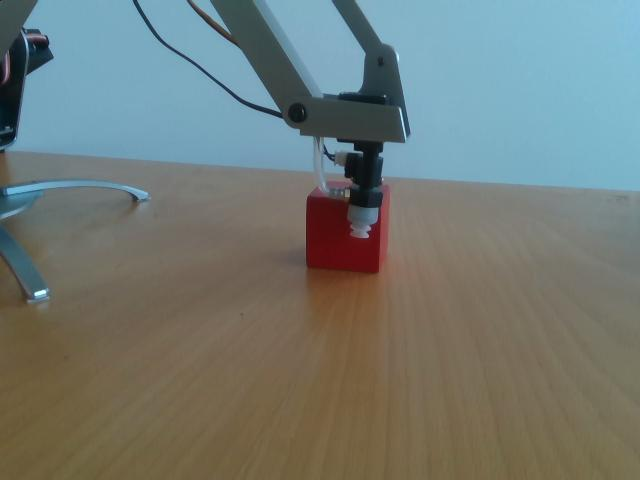
\includegraphics[width=0.3 \textwidth]{res/spiderman1.jpg}
    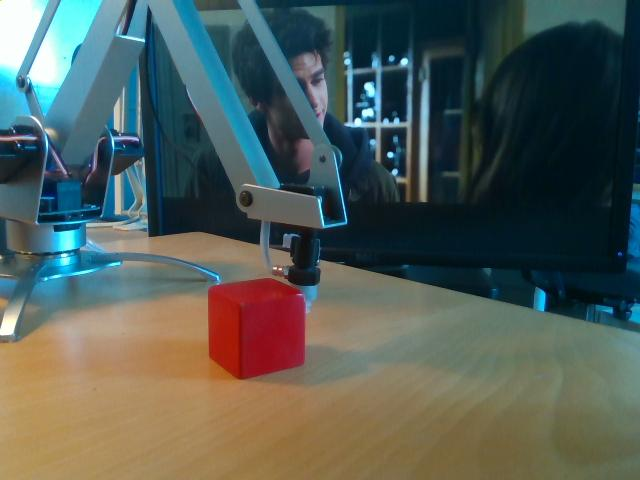
\includegraphics[width=0.3 \textwidth]{res/spiderman2.jpg}
    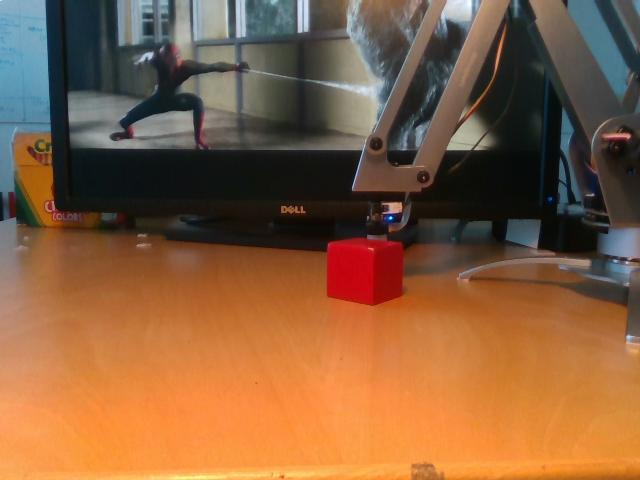
\includegraphics[width=0.3 \textwidth]{res/spiderman3.jpg}

    \caption{Data gathering for pose estimation in coordinate frame defined by
    the position and orientation of the end-effector. Camera was randomly
    placed at different positions, angles, and heights. To make predictions
    robust, images were recorded using different lighting conditions, different
    table surfaces, and different backgrounds.}

    \label{fig:relpose-training-data}
    
\end{figure}

\section{Results}

Plotting the labels against the predicted values show that the network can
learn the relative poses, albeit the precision being roughly $\pm 1$ cm was not
good enough to get robust results on the robots. Plots of labels plotted
against predicted values are shown in figure \ref{fig:relpose_end2end_results}.
Roughly estimating the influence of the resolution gives the following: Assume
the cube is at such a distance that $8$ cubes fit next to each other while all
of them are still fitting inside the image borders. The input image has a width
of $340$ pixels, dividing the total width of $8$ cubes by the $340$ pixels
gives:

\begin{equation}
    4 \cdot 8 \text{ cm / } 340 \text{ pixels } \approx 0.09 \text{ cm / pixel } \approx 1 \text{ mm / pixel }
\end{equation}

The intermediary representation has half the resolution implying approximately
$2$ mm / pixel which can only to a small extent explain the noisy predictions.
On top of this, pose estimates were shown to vary approximately $\pm 5$ mm from
scan to scan, partially explaining the appearance of the plots in figure
\ref{fig:relpose_end2end_results}. The fact remains though that when running
estimation on one of the real robots, it failed to give stable results.

\begin{figure}[h!]
    \centering
    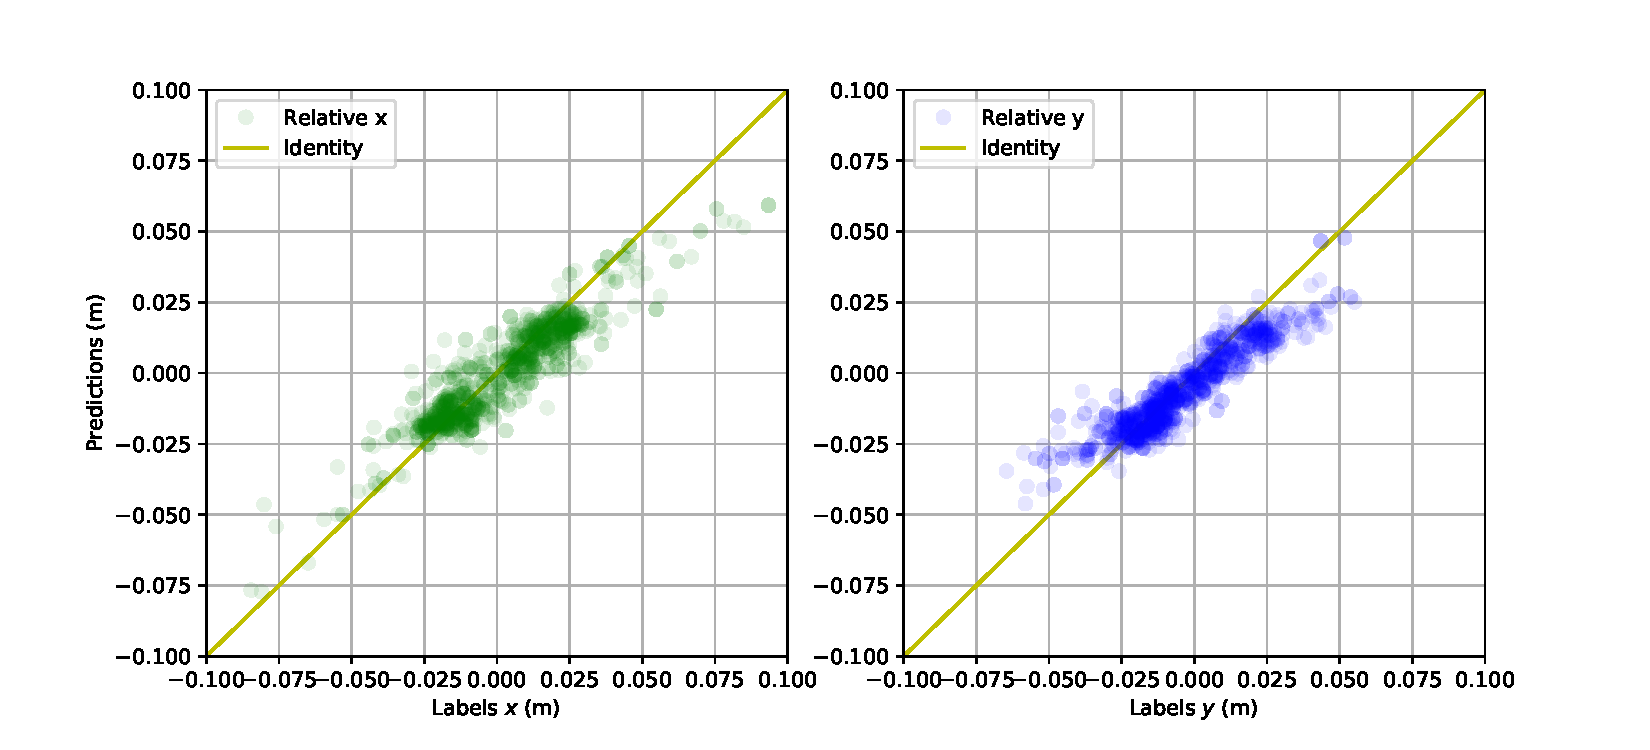
\includegraphics[width=0.8 \textwidth]{res/results_relative_pose_end2end.pdf}

    \caption{Results for estimating the cube pose in the end-effector frame using
    RGB-images from a camera at random positions, heights, and orientations. Target values
    (horizontal axis) are plotted against predicted values (vertical axis). The model
    predictions were too inaccurate to produce good results on the robots for the
    pushing task.}

    \label{fig:relpose_end2end_results}
    
\end{figure}

